\documentclass{standalone}
\usepackage{tikz}
\tikzstyle{inarrow}=[->, >=stealth, shorten >=.03cm,line width=1.5]
\tikzstyle{outarrow}=[<-, >=stealth, shorten <=.03cm,line width=1.5]
\begin{document}
\scalebox{10}{
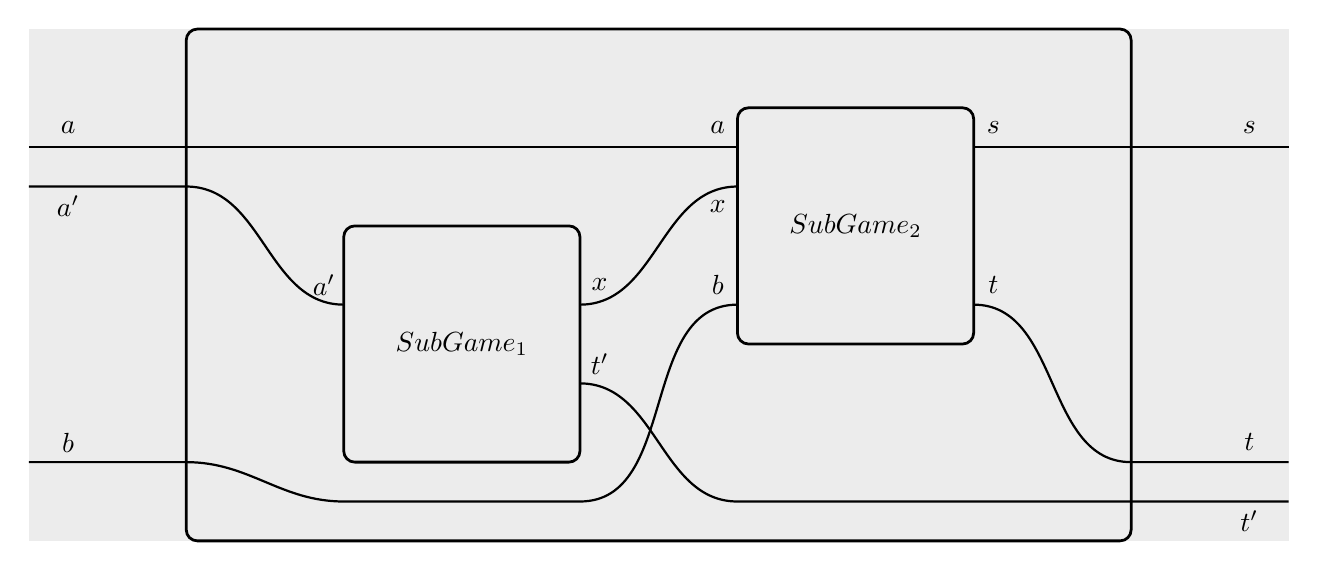
\begin{tikzpicture}
    \fill[gray!15] (-8,-4) rectangle (8,2.5);

    \draw[line width=1pt, rounded corners] (-6,-4) rectangle (6,2.5);
    \draw[line width=1pt, rounded corners] (-4,-3) rectangle (-1,0);
    \draw[line width=1pt, rounded corners] (1,-1.5) rectangle (4,1.5);

    % input
    \draw[thick] (-8,1) -- (1,1);
        \node (ao) at (-7.5,1.25) {$a$};
        \node (ai) at (0.75,1.25) {$a$};
    \draw[thick, in=180, out=0] (-8,0.5) to (-6,0.5) to (-4,-1);
        \node (ao') at (-7.5,.25) {$a'$};
        \node (ai') at (-4.25,-.75) {$a'$};
    \draw[thick, in=180, out=0] (-1,-1) to (1,0.5);
        \node (x) at (-.75,-.75) {$x$};
        \node (x) at (.75,0.25) {$x$};
    % feedback
    \draw[thick, in=180, out=0] (-8,-3) to (-6,-3) to (-4,-3.5) to (-1,-3.5) to (1,-1);
        \node (bi) at (-7.5,-2.75) {$b$};
        \node (bo) at (0.75,-.75) {$b$};
        
    % output
    \draw[thick, in=180, out=0] (4,1) to (6,1) to (8,1);
        \node (si) at (4.25,1.25) {$s$};
        \node (so) at (7.5,1.25) {$s$};

    % return
    \draw[thick, in=180, out=0] (-1,-2) to (1,-3.5) to (6,-3.5) to (8,-3.5);
    \draw[thick, in=180, out=0] (4,-1) to (6,-3) to (8,-3);
        \node (to) at (7.5,-2.75) {$t$};
        \node (to') at (7.5,-3.75) {$t'$};    
        \node (ti') at (-.75,-1.75) {$t'$};
        \node (to') at (4.25,-.75) {$t$};

    % content
        \node (X) at (-2.5,-1.5) {$SubGame_1$};    
        \node (Y) at (2.5,0) {$SubGame_2$};
        
\end{tikzpicture}}
\end{document}